\documentclass[11pt]{article}

\usepackage[margin=1in]{geometry}
\usepackage{graphicx}

\begin{document}
\title{Quantitative Formal Methods\\Modelling Speedoo}
\author{Renan Greca}
\maketitle

\section*{Introduction}
Speedoo, introduced in the article [...], is a tool designed to help software developers find optimization opportunities in large-scale programs.
Instead of just outputting a list of methods that should be optimized, the core of the Speedooo solution lies on the concept of \textit{optimization spaces}, each of which is a set of related methods that together provide one optimization opportunity.

For example, if two methods $f$ and $g$ are reasonably fast in isolation, a traditional tool might not suggest them as optimization opportunities.
However, if $f$ calls $g$ multiple times during execution, $f$ and $g$ form an optimization space and should be analyzed by the developers together -- perhaps there is a way of optimizing the number of calls to $g$ within $f$.

\section*{Modelling Speedoo}
To analyze Speedoo, a petri net was designed using the steps taken by the tool as a general guide of the places and transitions of the network.
Figure 2 from the Speedoo article provides the steps, complemented by Table 8, also from Speedoo, which provides the performance overhead of each step.

\begin{figure*}[!htbp]
\centering
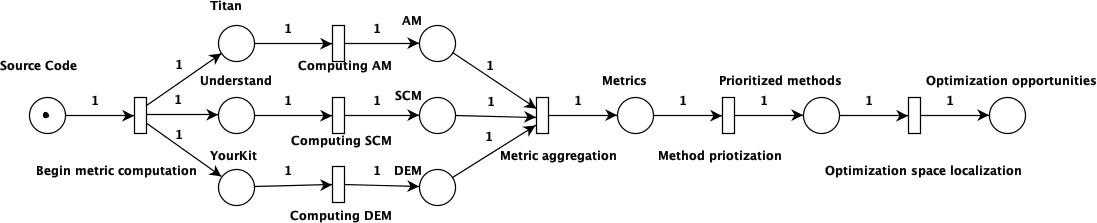
\includegraphics[scale=0.4]{speedoo_petrinet.png}
\caption{The shortest possible path in a 3x3 grid.}
\label{fig:vacuum3x3}
\end{figure*}

\begin{thebibliography}{99}
 
\bibitem{none} Chen Z, Chen B, Xiao L, Wang X, Chen L, Liu Y, Xu B (2018), \textquotedblleft Speedoo: Prioritizing Performance Optimization Opportunities Zhifei,\textquotedblright\ \textit{Proceedings of the 40th International Conference on Software Engineering  - ICSE '18}.

\end{thebibliography}


\end{document}
